%!TEX root = ../../../report.tex

\begin{figure}[H]
    \newcommand{\figurewidth}{0.496\textwidth}
    \newcommand{\figureheight}{4cm}
	\centering
	\begin{subfigure}[b]{\figurewidth}
        \figureborder{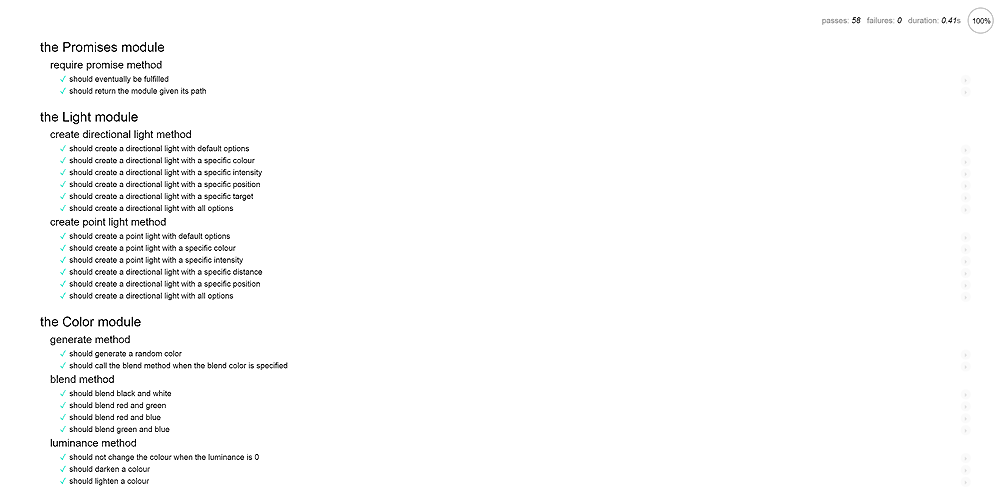
\includegraphics[width=\textwidth,height=\figureheight]{images/testing/mocha_before}}
        \caption{Default Mocha interface.}
        \label{fig:mocha_before}
    \end{subfigure}
    \begin{subfigure}[b]{\figurewidth}
        \figureborder{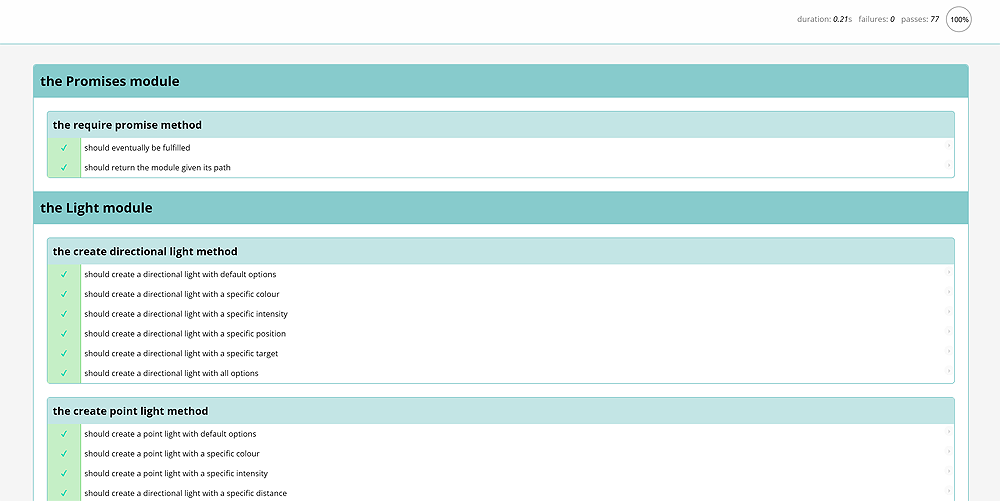
\includegraphics[width=\textwidth,height=\figureheight]{images/testing/mocha_after}}
        \caption{Mocha interface after custom styling}
        \label{fig:mocha_after}
    \end{subfigure}
	\caption[Mocha]{Mocha styling}
	\label{fig:mocha_styling}
\end{figure}
